\section{Discussions}\label{discussion}

Compared with the SS ADCs, the SAR/SS ADCs relatively require fewer extra control circuits to achieve adaptive-precision and take fewer steps to complelte the conversion. However, the SS ADCs inherently require less area and are easier to design. Therefore, depending on the specific design specifications, different architectures can be selected. 

As for the proportion between the power-off time and the total conversion time, 64/78 is achieved in the SAR/SS ADCs, which is a little less than the number 240/256 in the SS ADCs. More generally, assume that the low-precision conversion targets $a$ bits and the full-presision conversion targets $b$ bits, the corresponding equations to formulate the achievable proportion of the power-off time for the SS ADCs and SAR/SS ADCs would be as $(2^b-2^a)/2^b$ and $2^{b-a}/(k*a+2^{b-a})$, where $k$ is a coefficient describing how many extra steps are needed for the comparisons with SAR logic.
The closer this proportion is to 1, the better power scaling performance can be obtained.

Further assuming $k=3$, we can plot the achievable proportion of the power-off time for the SS ADCs and SAR/SS ADCs with different $a$ and $b$ as in Fig.~\ref{Proportion}. 
It shows that given the same full-precision bits, the SS ADCs will always have better power scaling capability than SAR/SS ADCs for different low-precision bits. However, in the cases where $b-a$ is relatively large, the gaps of power scaling capability between the SAR/SS and SS ADCs will be quite small. On the other hand, the SS ADCs naturally have trouble converting with higher than 10 bits because exponentially increasing conversion steps would severely limit throuput. 
Therefore, referring to the two black stars in Fig.~\ref{Proportion}, it is reasonable to adopt 4/8-bit adaptive-precision for the SS ADCs and 4/10-bit adaptive-precision for SAR/SS ADCs with a trade-off between the throuput limitation and power scaling capability.

\begin{figure}[htbp]
	\centerline{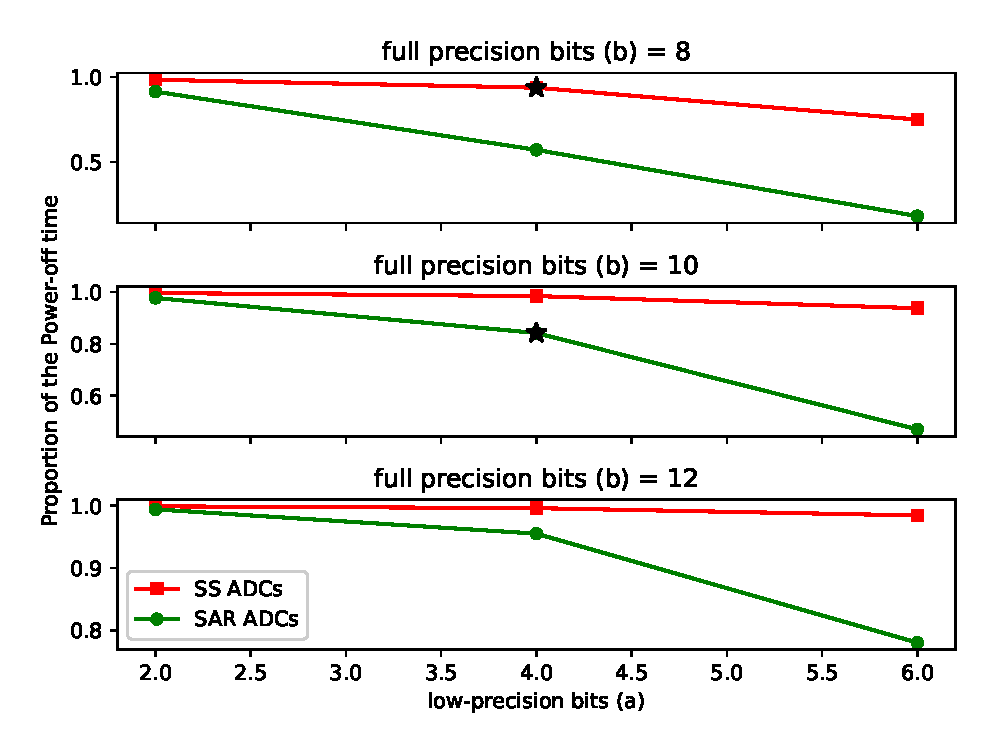
\includegraphics[width=3.5in]{./Figures/Proportion.eps}}
	\caption{Achievable Proportion of the Power-off time for the SS and SAR/SS ADCs.}
	\label{Proportion}
\end{figure} 

For other different precision configurations and number of parallel collumns, 
the corresponding power consumption and energy-saving performance can also be estimated by extending the evaluation results in Sect.~\ref{result}.